\documentclass[]{article}
\usepackage{amssymb,amsmath}
\usepackage{ifxetex,ifluatex}
\ifxetex
  \usepackage{fontspec,xltxtra,xunicode}
  \defaultfontfeatures{Mapping=tex-text,Scale=MatchLowercase}
\else
  \ifluatex
    \usepackage{fontspec}
    \defaultfontfeatures{Mapping=tex-text,Scale=MatchLowercase}
  \else
    \usepackage[utf8]{inputenc}
  \fi
\fi
\usepackage{color}
\usepackage{fancyvrb}
\DefineShortVerb[commandchars=\\\{\}]{\|}
\DefineVerbatimEnvironment{Highlighting}{Verbatim}{commandchars=\\\{\}}
% Add ',fontsize=\small' for more characters per line
\newenvironment{Shaded}{}{}
\newcommand{\KeywordTok}[1]{\textcolor[rgb]{0.00,0.44,0.13}{\textbf{{#1}}}}
\newcommand{\DataTypeTok}[1]{\textcolor[rgb]{0.56,0.13,0.00}{{#1}}}
\newcommand{\DecValTok}[1]{\textcolor[rgb]{0.25,0.63,0.44}{{#1}}}
\newcommand{\BaseNTok}[1]{\textcolor[rgb]{0.25,0.63,0.44}{{#1}}}
\newcommand{\FloatTok}[1]{\textcolor[rgb]{0.25,0.63,0.44}{{#1}}}
\newcommand{\CharTok}[1]{\textcolor[rgb]{0.25,0.44,0.63}{{#1}}}
\newcommand{\StringTok}[1]{\textcolor[rgb]{0.25,0.44,0.63}{{#1}}}
\newcommand{\CommentTok}[1]{\textcolor[rgb]{0.38,0.63,0.69}{\textit{{#1}}}}
\newcommand{\OtherTok}[1]{\textcolor[rgb]{0.00,0.44,0.13}{{#1}}}
\newcommand{\AlertTok}[1]{\textcolor[rgb]{1.00,0.00,0.00}{\textbf{{#1}}}}
\newcommand{\FunctionTok}[1]{\textcolor[rgb]{0.02,0.16,0.49}{{#1}}}
\newcommand{\RegionMarkerTok}[1]{{#1}}
\newcommand{\ErrorTok}[1]{\textcolor[rgb]{1.00,0.00,0.00}{\textbf{{#1}}}}
\newcommand{\NormalTok}[1]{{#1}}
\usepackage{graphicx}
% We will generate all images so they have a width \maxwidth. This means
% that they will get their normal width if they fit onto the page, but
% are scaled down if they would overflow the margins.
\makeatletter
\def\maxwidth{\ifdim\Gin@nat@width>\linewidth\linewidth
\else\Gin@nat@width\fi}
\makeatother
\let\Oldincludegraphics\includegraphics
\renewcommand{\includegraphics}[1]{\Oldincludegraphics[width=8cm]{#1}}
\ifxetex
  \usepackage[setpagesize=false, % page size defined by xetex
              unicode=false, % unicode breaks when used with xetex
              xetex,
              colorlinks=true,
              linkcolor=blue]{hyperref}
\else
  \usepackage[unicode=true,
urlcolor=blue,
              colorlinks=true,
              linkcolor=blue]{hyperref}
\fi
\hypersetup{breaklinks=true, pdfborder={0 0 0}}
\setlength{\parindent}{0pt}
\setlength{\parskip}{6pt plus 2pt minus 1pt}
\setlength{\emergencystretch}{3em}  % prevent overfull lines
\setcounter{secnumdepth}{0}

\pagestyle{myheadings}
\author{Lovelace, Robin\\
\texttt{r.lovelace@leeds.ac.uk}
\and
Cheshire, James\\
\texttt{james.cheshire@ucl.ac.uk}
}
\title{Introduction to visualising spatial data in R}
\markboth{\hfill }{GeoTALISMAN Short Course \hfill}
\usepackage[margin=2cm]{geometry}

\begin{document}
\maketitle

\section{Introduction}

This tutorial is an introduction to spatial data in R and map making
with the popular graphics package \texttt{ggplot2}. It assumes no prior
knowledge of spatial data analysis but prior understanding of R command
line would be beneficial. For people new to R, we recommend working
through an `Introduction to R' type tutorial, such as ``A (very) short
introduction to R''
(\href{http://cran.r-project.org/doc/contrib/Torfs+Brauer-Short-R-Intro.pdf}{Torfs
and Brauer, 2012}) or the more geographically inclined ``Short
introduction to R''
(\href{http://www.social-statistics.org/wp-content/uploads/2012/12/intro\_to\_R1.pdf}{Harris,
2012}).

Building on such background material, the following set of exercises is
concerned with specific functions for spatial data and visualisation. An
up-to-date version of this tutorial is maintained at
\href{https://github.com/Robinlovelace/Creating-maps-in-R/blob/master/intro-spatial-rl.pdf}{https://github.com/Robinlovelace/Creating-maps-in-R}
and the entire tutorial, including the input data can be downloaded as a
\href{https://github.com/Robinlovelace/Creating-maps-in-R/archive/master.zip}{zip
file}, as described below. Suggested improvements welcome - please
\href{https://help.github.com/articles/fork-a-repo}{fork}, improve and
push this document to its original home to ensure its longevity.

\subsection{Typographic conventions and getting help}

To ensure reproducibility and allow automatic syntax highlighting, this
document has been written in RMarkdown. We try to follow best practice
in terms of style, roughly following Google's style guide and the
excellent ``Rchaeological Commentary''
(\href{http://cran.r-project.org/web/packages/rockchalk/vignettes/Rstyle.pdf}{Johnson
2013}). It is a good idea to get into the habit of consistent and clear
writing in any language, and R is no exception. Adding comments to your
code is also good practice, so you remember at a later date what you've
done, aiding the learning process. There are two main ways of commenting
code using the \texttt{\#} symbol: above a line of code or directly
following it, as illustrated below.

\begin{Shaded}
\begin{Highlighting}[]
\CommentTok{# Generate data}
\NormalTok{x <- }\DecValTok{1}\NormalTok{:}\DecValTok{400}
\NormalTok{y <- }\KeywordTok{sin}\NormalTok{(x/}\DecValTok{10}\NormalTok{) * }\KeywordTok{exp}\NormalTok{(x * -}\FloatTok{0.01}\NormalTok{)}

\KeywordTok{plot}\NormalTok{(x, y)  }\CommentTok{# plot the result}
\end{Highlighting}
\end{Shaded}
In the above code we first created a new \emph{object} that we have
called \texttt{x}. Any name could have been used, like \texttt{xBumkin},
but \texttt{x} works just fine here, although it is good practice to
give your objects meaningful names. Note the use of the
\texttt{\textless{}-} ``arrow'' symbol, which tells R to create a new
object. We will be using this symbol a lot in the tutorial. Each time it
is used, a new object is created (or an old one is overwritten).

Be aware of the following typographic conventions: R code (e.g.
\texttt{plot(x, y)}) is written in a \texttt{monospace} font while prose
is not. Blocks of code such as,

\begin{Shaded}
\begin{Highlighting}[]
\KeywordTok{c}\NormalTok{(}\DecValTok{1}\NormalTok{:}\DecValTok{3}\NormalTok{, }\DecValTok{5}\NormalTok{)^}\DecValTok{2}
\end{Highlighting}
\end{Shaded}
\begin{verbatim}
## [1]  1  4  9 25
\end{verbatim}
are compiled in-line: the \texttt{\#\#} indicates this is output from R.
Some of the output from the code below is quite long so we only show the
output that is useful - it should also be clear when we have decided to
omit an image from this document to save space. All images in this
document are small and low-quality to save space; they should display
better on your computer screen and can be saved at any resolution. The
code presented here is not the only way to do things: we encourage you
to play with it and try things out to gain a deeper understanding of R.
Don't worry, you cannot `break' anything using R and all the input data
can be re-loaded if things do go wrong.

If you require help on any function, use the \texttt{help} function,
e.g. \texttt{help(plot)}. Because R users love being concise, this can
also be written as \texttt{?plot}. We will suggest when looking at this
help may be useful in the tutorial, but feel free to use it at any point
you'd like more detail (although R's help files are famously cryptic for
the un-initiated). For the most part, \emph{learning by doing} is a good
motto, so let's crack on and download some packages and then some data.

\subsection{Prerequisites and packages}

For this tutorial you need to install R, the latest version of which can
be downloaded from
\href{http://cran.r-project.org/}{http://cran.r-project.org/}. A number
of R editors such as \href{http://www.rstudio.com/}{RStudio} can be used
to make R more user friendly, but these are not needed to complete the
tutorial.

R has a huge and growing number of spatial data packages. These can be
installed in one go with the \texttt{ctv} package and the command
\texttt{install.views("Spatial")}. We do NOT recommend running this
command for this tutorial: partly because downloading and compiling all
spatial packages takes a long time (hundreds of megabytes) and also
because we will add new packages when they are needed to see what each
does. We do recommend taking a quick browse at the range of spatial
packages on offer though:
\href{http://cran.r-project.org/web/views/Spatial.html}{http://cran.r-project.org/web/views/Spatial.html}.

The packages we will be using are \texttt{ggplot2}, \texttt{rgdal},
\texttt{rgeos}, \texttt{maptools} and \texttt{ggmap}. To test whether
ggplot2 is installed, for example, enter \texttt{library(ggplot2)}. If
you get an error message, it needs to be installed:
\texttt{install.packages("ggplot2")}. These will be downloaded from CRAN
(the Comprehensive R Archive Network); if you are prompted to select a
`mirror', select one that is close to your city.

\subsection{Downloading the data for the tutorial}

The data used for the tutorial can be downloaded from
\href{https://github.com/Robinlovelace/Creating-maps-in-R}{https://github.com/Robinlovelace/Creating-maps-in-R}.
Click on the ``Download ZIP'' button on the right and unzip this to a
new folder. Use the \texttt{setwd} command to set the working directory.
If your username is ``username'' and you saved the files into a folder
called ``Creating-maps-in-R-master'' on your Desktop, for example, you
would type the following:

\begin{Shaded}
\begin{Highlighting}[]
\KeywordTok{setwd}\NormalTok{(}\StringTok{"C:/Users/username/Desktop/Creating-maps-in-R-master/"}\NormalTok{)}
\end{Highlighting}
\end{Shaded}
If you are working in RStudio, you can create a project that will
automatically set your working directory.

\section{Loading and interrogating spatial data}

One of the most important steps in handling spatial data with R is the
ability to read in shapefiles. There are a number of ways to do this,
the most commonly used and versatile of which is \texttt{readOGR}. This
function, from the \texttt{rgdal} package, automatically extracts
information about the projection and the attributes of data.
\texttt{rgdal} is R's interface to the ``Geospatial Abstraction Library
(GDAL)'' which is used by other open source GIS packages such as QGIS
and enables R to handle a broader range of spatial data formats.

\begin{Shaded}
\begin{Highlighting}[]
\KeywordTok{library}\NormalTok{(rgdal)}
\NormalTok{sport <- }\KeywordTok{readOGR}\NormalTok{(}\DataTypeTok{dsn =} \StringTok{"data"}\NormalTok{, }\StringTok{"london_sport"}\NormalTok{)}
\end{Highlighting}
\end{Shaded}
\begin{verbatim}
## OGR data source with driver: ESRI Shapefile 
## Source: "data", layer: "london_sport"
## with 33 features and 4 fields
## Feature type: wkbPolygon with 2 dimensions
\end{verbatim}
In the code above \texttt{dsn} stands for ``data source name'' and is an
\emph{argument} of the \emph{function} \texttt{readOGR}. The
\texttt{dsn} argument this case, specifies the directory in which the
dataset is stored. R functions have a default order of arguments, so
\texttt{dsn =} does not actually need to be typed. If there data were
stored in the current working directory, one could use
\texttt{readOGR(".", "london\_sport")}. For clarity, it is good practice
to include argument names, such as \texttt{dsn} when learning new
functions.

The next argument is a \emph{character string}. This is simply the name
the file required. There is no need to add a file extension (e.g.
\texttt{.shp}) in this case. The files beginning \texttt{london\_sport}
from the
\href{http://spatial.ly/wp-content/uploads/2013/12/spatialggplot.zip}{example
dataset} contain the borough population and the percentage of the
population engaging in sporting activities and was taken from the
\href{http://data.london.gov.uk/datastore/package/active-people-survey-kpi-data-borough}{active
people survey}. The boundary data is from the
\href{http://www.ordnancesurvey.co.uk/oswebsite/opendata/}{Ordnance
Survey}.

Now that we have a spatial object loaded into R's workspace, we can try
analysing it with some basic commands:

\begin{Shaded}
\begin{Highlighting}[]
\KeywordTok{head}\NormalTok{(sport@data, }\DataTypeTok{n =} \DecValTok{2}\NormalTok{)}
\end{Highlighting}
\end{Shaded}
\begin{verbatim}
##   ons_label                 name Partic_Per Pop_2001
## 0      00AF              Bromley       21.7   295535
## 1      00BD Richmond upon Thames       26.6   172330
\end{verbatim}
\begin{Shaded}
\begin{Highlighting}[]
\KeywordTok{mean}\NormalTok{(sport$Partic_Per)}
\end{Highlighting}
\end{Shaded}
\begin{verbatim}
## [1] 20.05
\end{verbatim}
There are two important symbols at work in the above block of code: the
\texttt{@} symbol is used to refer to the attribute \emph{slot} of the
dataset; the \texttt{\$} symbol refers to a specific variable,
identified from the result of running the first line. If you are using
RStudio, test out the autocompletion functionality by hitting
\texttt{tab} before completing the command - this can save you a lot of
time in the long run.

The \texttt{head} function in first line of the code above means ``show
the first few lines of data''. It's default is to output the first 6
lines (try simply \texttt{head(sport@data)}), but this is a bit much so
we have specified the number of lines \emph{argument} with
\texttt{n = 2}. The second line of code calculates the mean value of the
variable \texttt{Partic\_Per} (sports participation per 100 people) for
each of the zones in the spatial dataset. To test another function, try
typing \texttt{nrow(sport)} and record how many zones the dataset
contains.

Now we have seen something of the \emph{attributes} of the spatial
dataset, let us take a plot its \emph{geometry} data, which describes
where the polygons are located in space:

\begin{figure}[htbp]
\centering
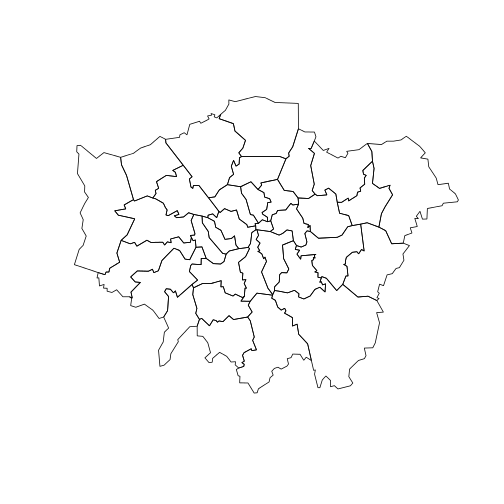
\includegraphics{figure/unnamed-chunk-6.png}
\caption{unnamed-chunk-6}
\end{figure}

\texttt{plot} is one of the most useful functions in R, as it is
\emph{polymorphic} meaning its behaviour changes depending on the input
data. Inputing another dataset (e.g. \texttt{plot(sport@data))} will
generate an entirely different type of plot altogether. Thus R is
intelligent at guessing what you want to do with the data you provide it
with.

R has powerful subsetting capabilities that can be accessed very
concisely using square brackets, as shown in the following example:

\begin{Shaded}
\begin{Highlighting}[]
\NormalTok{sport@data[sport$Partic_Per < }\DecValTok{15}\NormalTok{, ]}
\end{Highlighting}
\end{Shaded}
\begin{verbatim}
##    ons_label           name Partic_Per Pop_2001
## 17      00AQ         Harrow       14.8   206822
## 21      00BB         Newham       13.1   243884
## 32      00AA City of London        9.1     7181
\end{verbatim}
The above line of code asked R to select only those rows with very low
sports participation, in this case Harrow, Newham and the city centre.
The square brackets work as follows: anything before the comma refers to
the rows that will be selected, anything after the comma refers to the
columns. Try experimenting with this square brackets notation
(e.g.~guess the result of \texttt{sport@data{[}1:2, 1:3{]}} and test
it): it will be useful.

In the previous code example we have been interrogating only the
attribute data (hence \texttt{@data}) of the \texttt{sport} object, but
the square brackets can also be used to subset spatial datasets. Using
the same logic as before try to plot a subset of zones with high sports
participation.

\begin{Shaded}
\begin{Highlighting}[]
\KeywordTok{plot}\NormalTok{(sport[sport$Partic_Per > }\DecValTok{25}\NormalTok{, ])  }\CommentTok{# not shown in tutorial}
\end{Highlighting}
\end{Shaded}
\begin{figure}[htbp]
\centering
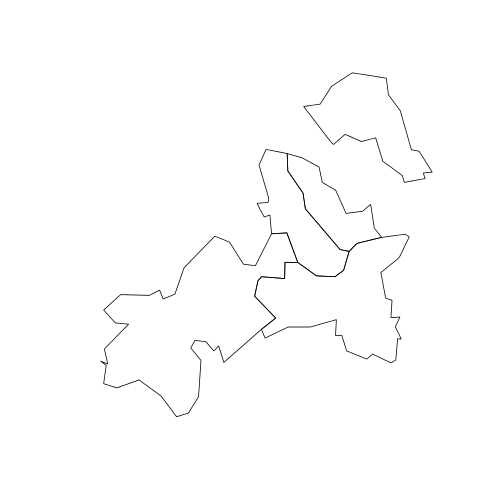
\includegraphics{figure/unnamed-chunk-8.png}
\caption{unnamed-chunk-8}
\end{figure}

This is useful, but it would be great to see these sporty areas in
context. To do this, simply use the \texttt{add = TRUE} argument after
the initial plot. (\texttt{add = T} would also work, but we like to
spell things out in this tutorial for clarity). What does the
\texttt{col} argument refer to in the below block - it should be
obvious!

\begin{Shaded}
\begin{Highlighting}[]
\KeywordTok{plot}\NormalTok{(sport)}
\KeywordTok{plot}\NormalTok{(sport[sport$Partic_Per > }\DecValTok{25}\NormalTok{, ], }\DataTypeTok{col =} \StringTok{"blue"}\NormalTok{, }\DataTypeTok{add =} \OtherTok{TRUE}\NormalTok{)}
\end{Highlighting}
\end{Shaded}
\begin{figure}[htbp]
\centering
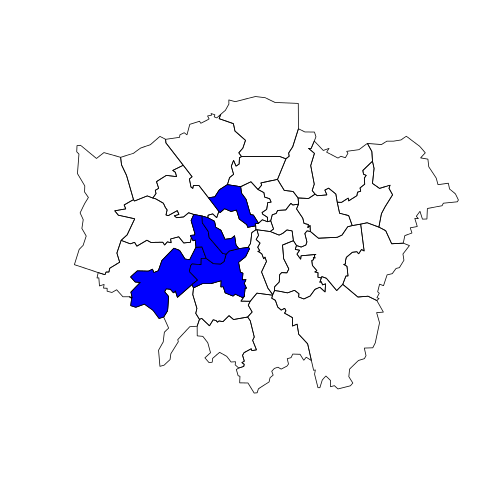
\includegraphics{figure/Preliminary_plot_of_London__Areas_with_high_sports_participation_are_blue.png}
\caption{Preliminary plot of London. Areas with high
sports participation are blue}
\end{figure}

Congratulations! You have just interrogated and visualised a spatial
dataset: what kind of places have high levels of sports participation?
The map tells us. Do not worry for now about the intricacies of how this
was achieved: you have learned vital basics of how R works as a
language; we will cover details this subsequent sections.

While we are on the topic of loading data, it is worth pointing out that
R can save and load data efficiently into its own data format
(\texttt{.RData}). Try \texttt{save(sport, file = "sport.RData")} and
see what happens. If you type \texttt{rm(sport)} (which removes the
object) and then \texttt{load("sport.RData")} you should see how this
works. \texttt{sport} will disappear from the workspace and then
reappear.

\subsection{Attribute data}

All shapefiles have both attribute table and geometry data. These are
automatically loaded with \texttt{readOGR}. The loaded attribute data
can be treated in a similar way to an R
\href{http://www.statmethods.net/input/datatypes.html}{data frame}.

R delibrately hides the geometry of spatial data unless you print the
entire object (try typing \texttt{print(sport)}). Let's take a look at
the headings of sport, using the following command:
\texttt{names(sport)} The data contained in spatial data are kept in a
`slot' that can be accessed using the @ symbol: \texttt{sport@data}.
This is useful if you do not wish to work with the spatial components of
the data at all times.

Type \texttt{summary(sport)} to get some additional information about
the data object. Spatial objects in R contain a variety of additional
information:

\begin{verbatim}
Object of class SpatialPolygonsDataFrame
Coordinates:
       min      max
x 503571.2 561941.1
y 155850.8 200932.5
Is projected: TRUE 
proj4string :
[+proj=tmerc +lat_0=49 +lon_0=-2 +k=0.9996012717 ....]
\end{verbatim}
\section{Manipulating spatial data in R}

It is all very well being able to load and interrogate spatial data in
R, but to compete with modern GIS packages it must also be able to
modify these spatial objects before they are visualised (see
`\href{https://github.com/Pakillo/R-GIS-tutorial}{using R as a GIS}'). R
has a wide range of very powerful functions for this, many of which are
in additional packages alluded to in the introduction.

This course is introductory so only the most commonly required data
manipulation tasks, \emph{reprojecting} and \emph{joining/clipping} are
covered here. We will look at joining aspatial datasets to our spatial
object via an attribute join. Spatial joins, whereby data is added to
the target layer depending on the location of the origins is also
covered.

\subsection{Changing projection}

You may have noticed the word \texttt{proj4string} in the summary of
\texttt{sport}. This represents the coordinate reference system used in
the data. In this file it has been incorrectly specified so we can
change it with the following:

\begin{Shaded}
\begin{Highlighting}[]
\KeywordTok{proj4string}\NormalTok{(sport) <- }\KeywordTok{CRS}\NormalTok{(}\StringTok{"+init=epsg:27700"}\NormalTok{)}
\end{Highlighting}
\end{Shaded}
\begin{verbatim}
## Warning: A new CRS was assigned to an object with an existing CRS:
## +proj=tmerc +lat_0=49 +lon_0=-2 +k=0.9996012717 +x_0=400000 +y_0=-100000 +ellps=airy +units=m +no_defs
## without reprojecting.
## For reprojection, use function spTransform in package rgdal
\end{verbatim}
You will see a warning. This is simply saying that you are changing the
coordinate reference system, not reprojecting the data. Epsg:27700 is
the code for British National Grid. If we wanted to reproject the data
into something like WGS84 for latitude and longitude we would use the
following code:

\begin{Shaded}
\begin{Highlighting}[]
\NormalTok{sport.wgs84 <- }\KeywordTok{spTransform}\NormalTok{(sport, }\KeywordTok{CRS}\NormalTok{(}\StringTok{"+init=epsg:4326"}\NormalTok{))}
\end{Highlighting}
\end{Shaded}
The different epsg codes are a bit of hassle to remember but you can
find them all at
\href{http://spatialreference.org/}{spatialreference.org}.

\subsection{Attribute joins}

To reaffirm our starting point, let's re-load the spatial data and plot
it. We will call this new object \texttt{lnd}, short for London:

\begin{Shaded}
\begin{Highlighting}[]
\KeywordTok{library}\NormalTok{(rgdal)}
\NormalTok{lnd <- }\KeywordTok{readOGR}\NormalTok{(}\DataTypeTok{dsn =} \StringTok{"data"}\NormalTok{, }\StringTok{"london_sport"}\NormalTok{)}
\end{Highlighting}
\end{Shaded}
\begin{verbatim}
## OGR data source with driver: ESRI Shapefile 
## Source: "data", layer: "london_sport"
## with 33 features and 4 fields
## Feature type: wkbPolygon with 2 dimensions
\end{verbatim}
\begin{Shaded}
\begin{Highlighting}[]
\KeywordTok{plot}\NormalTok{(lnd)}
\end{Highlighting}
\end{Shaded}
\begin{figure}[htbp]
\centering
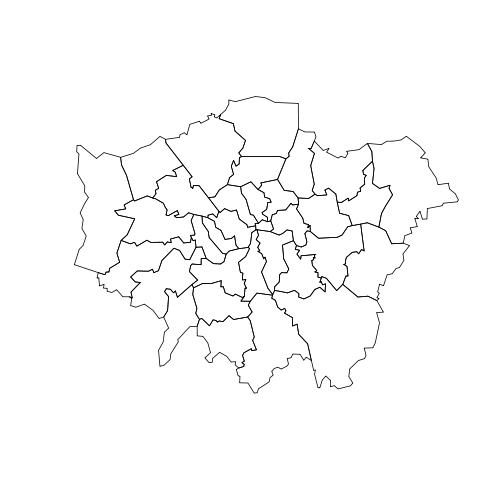
\includegraphics{figure/Plot_of_London.png}
\caption{Plot of London}
\end{figure}

\begin{Shaded}
\begin{Highlighting}[]
\KeywordTok{nrow}\NormalTok{(lnd)}
\end{Highlighting}
\end{Shaded}
\begin{verbatim}
## [1] 33
\end{verbatim}
The dataset we will join to the London object is a dataset on recorded
crimes, with one row per crime. We will use the non-spatial
implementation of \texttt{aggregate} to pre-process this dataset ready
to join to our spatial \texttt{lnd} dataset.

\begin{Shaded}
\begin{Highlighting}[]
\NormalTok{crimeDat <- }\KeywordTok{read.csv}\NormalTok{(}\StringTok{"data/mps-recordedcrime-borough.csv"}\NormalTok{, }\DataTypeTok{fileEncoding =} \StringTok{"UCS-2LE"}\NormalTok{)}
\KeywordTok{head}\NormalTok{(crimeDat)}
\KeywordTok{summary}\NormalTok{(crimeDat$MajorText)}
\NormalTok{crimeTheft <- crimeDat[}\KeywordTok{which}\NormalTok{(crimeDat$MajorText == }\StringTok{"Theft & Handling"}\NormalTok{), ]}
\KeywordTok{head}\NormalTok{(crimeTheft, }\DecValTok{2}\NormalTok{)  }\CommentTok{# change 2 for more rows}
\NormalTok{crimeAg <- }\KeywordTok{aggregate}\NormalTok{(CrimeCount ~ Spatial_DistrictName, }\DataTypeTok{FUN =} \StringTok{"sum"}\NormalTok{, }\DataTypeTok{data =} \NormalTok{crimeTheft)}
\KeywordTok{head}\NormalTok{(crimeAg, }\DecValTok{2}\NormalTok{)  }\CommentTok{# show the aggregated crime data}
\end{Highlighting}
\end{Shaded}
Now that we have crime data at the borough level, the challenge is to
join it by name. This is not always straightforward. Let us see which
names in the crime data match the spatial data:

\begin{Shaded}
\begin{Highlighting}[]
\NormalTok{lnd$name %in% crimeAg$Spatial_DistrictName}
\end{Highlighting}
\end{Shaded}
\begin{verbatim}
##  [1]  TRUE  TRUE  TRUE  TRUE  TRUE  TRUE  TRUE  TRUE  TRUE  TRUE  TRUE
## [12]  TRUE  TRUE  TRUE  TRUE  TRUE  TRUE  TRUE  TRUE  TRUE  TRUE  TRUE
## [23]  TRUE  TRUE  TRUE  TRUE  TRUE  TRUE  TRUE  TRUE  TRUE  TRUE FALSE
\end{verbatim}
\begin{Shaded}
\begin{Highlighting}[]
\NormalTok{lnd$name[}\KeywordTok{which}\NormalTok{(!lnd$name %in% crimeAg$Spatial_DistrictName)]}
\end{Highlighting}
\end{Shaded}
\begin{verbatim}
## [1] City of London
## 33 Levels: Barking and Dagenham Barnet Bexley Brent Bromley ... Westminster
\end{verbatim}
The first line of code above shows that all but one of the borough names
matches; the second tells us that it is City of London, row 25, that is
named differently in the crime data. Look at the results (not shown
here) on your computer.

\begin{Shaded}
\begin{Highlighting}[]
\KeywordTok{levels}\NormalTok{(crimeAg$Spatial_DistrictName)}
\KeywordTok{levels}\NormalTok{(crimeAg$Spatial_DistrictName)[}\DecValTok{25}\NormalTok{] <- }\KeywordTok{as.character}\NormalTok{(lnd$name[}\KeywordTok{which}\NormalTok{(!lnd$name %in% }
    \NormalTok{crimeAg$Spatial_DistrictName)])}
\NormalTok{lnd$name %in% crimeAg$Spatial_DistrictName  }\CommentTok{# now all columns match}
\end{Highlighting}
\end{Shaded}
The above code block first identified the row with the faulty name and
then renamed the level to match the \texttt{lnd} dataset. Note that we
could not rename the variable directly, as it is stored as a factor.

We are now ready to join the datasets. It is recommended to use the
\texttt{join} function in the \texttt{plyr} package but the
\texttt{merge} function could equally be used.

\begin{Shaded}
\begin{Highlighting}[]
\KeywordTok{help}\NormalTok{(join)}
\KeywordTok{library}\NormalTok{(plyr)}
\KeywordTok{help}\NormalTok{(join)  }\CommentTok{# now help should appear}
\end{Highlighting}
\end{Shaded}
The documentation for join will be displayed if the plyr package is
loaded (if not, load or install and load it!). It requires all joining
variables to have the same name, so we will rename the variable to make
the join work:

\begin{Shaded}
\begin{Highlighting}[]
\KeywordTok{head}\NormalTok{(lnd$name)}
\KeywordTok{head}\NormalTok{(crimeAg$Spatial_DistrictName)  }\CommentTok{# the variables to join}
\NormalTok{crimeAg <- }\KeywordTok{rename}\NormalTok{(crimeAg, }\DataTypeTok{replace =} \KeywordTok{c}\NormalTok{(}\DataTypeTok{Spatial_DistrictName =} \StringTok{"name"}\NormalTok{))}
\KeywordTok{head}\NormalTok{(}\KeywordTok{join}\NormalTok{(lnd@data, crimeAg))  }\CommentTok{# test it works}
\end{Highlighting}
\end{Shaded}
\begin{verbatim}
## Joining by: name
\end{verbatim}
\begin{Shaded}
\begin{Highlighting}[]
\NormalTok{lnd@data <- }\KeywordTok{join}\NormalTok{(lnd@data, crimeAg)}
\end{Highlighting}
\end{Shaded}
\begin{verbatim}
## Joining by: name
\end{verbatim}
Take a look at the \texttt{lnd@data} object. You should see new
variables added, meaning the attribute join was successful.

\subsection{Spatial joins}

In addition to joining by zone name, it is also possible to do
\href{http://help.arcgis.com/en/arcgisdesktop/10.0/help/index.html\#//00080000000q000000}{spatial
joins} in R. There are three main varieties: many-to-one, where the
values of many intersecting objects contribute to a new variable in the
main table, one-to-many, or one-to-one. Because boroughs in London are
quite large, we will conduct a many-to-one spatial join. We will be
using Tube Stations as the spatial data to join, with the aim of finding
out which and how many stations are found in each London borough.

\begin{Shaded}
\begin{Highlighting}[]
\KeywordTok{library}\NormalTok{(rgdal)}
\NormalTok{stations <- }\KeywordTok{readOGR}\NormalTok{(}\DataTypeTok{dsn =} \StringTok{"data"}\NormalTok{, }\DataTypeTok{layer =} \StringTok{"lnd-stns"}\NormalTok{)}
\KeywordTok{proj4string}\NormalTok{(stations)  }\CommentTok{# this is the full geographical detail.}
\KeywordTok{proj4string}\NormalTok{(lnd)}
\KeywordTok{bbox}\NormalTok{(stations)}
\KeywordTok{bbox}\NormalTok{(lnd)}
\end{Highlighting}
\end{Shaded}
The above code loads the data correctly, but also shows that there are
problems with it: the Coordinate Reference System (CRS) of the stations
differs from that of our \texttt{lnd} object. OSGB 1936 (or
\href{http://spatialreference.org/ref/epsg/27700/}{EPSG 27700}) is the
official CRS for the UK, so we will convert the stations dataset to
this:

\begin{Shaded}
\begin{Highlighting}[]
\NormalTok{stations27700 <- }\KeywordTok{spTransform}\NormalTok{(stations, }\DataTypeTok{CRSobj =} \KeywordTok{CRS}\NormalTok{(}\KeywordTok{proj4string}\NormalTok{(lnd)))}
\NormalTok{stations <- stations27700}
\KeywordTok{rm}\NormalTok{(stations27700)  }\CommentTok{# cleaning up}
\KeywordTok{plot}\NormalTok{(lnd)}
\KeywordTok{points}\NormalTok{(stations)}
\end{Highlighting}
\end{Shaded}
\begin{figure}[htbp]
\centering
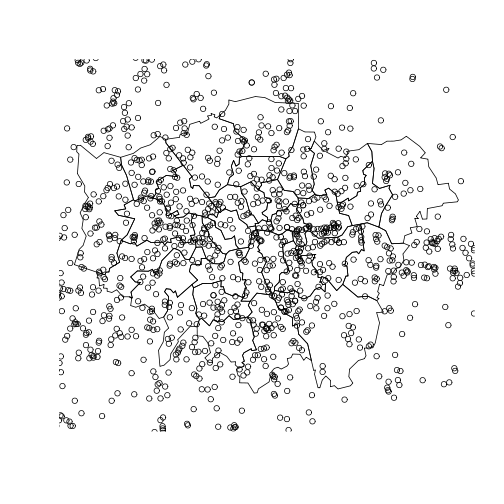
\includegraphics{figure/Sampling_and_plotting_stations.png}
\caption{Sampling and plotting stations}
\end{figure}

Now we can clearly see that the stations overlay the boroughs. The
problem is that the stations dataset is far more extensive than London
borough dataset; we take a spatially determined subset of the former so
that they all fit within the latter. This is \emph{clipping}.

\subsection{Clipping}

There are a number of functions that we can use to clip the points so
that only those falling within London boroughs are retained. These
include \texttt{overlay}, \texttt{sp::over}, and
\texttt{rgeos::gIntersects} (the word preceding the \texttt{::} symbol
refers to the package the function is from). Use \texttt{?} followed by
the function to get help on each and find which is most appropriate.
\texttt{gIntersects} can produce the same output as \texttt{over} for
basic joins (Bivand et al. 2013).

In this tutorial we will use the \texttt{over} function as it is easiest
to use. \texttt{gIntersects} can achieve the same result, but with more
lines of code. It may seem confusing that two different functions can be
used to generate the same result. However, this is a common issue in
programming; the question is finding the most appropriate solution.

\texttt{over} takes two main input arguments: the target layer to be
altered and the layer by which it is to be clipped. The output is a data
frame of the same dimensions as the original dataset, except that the
values corresponding to areas outside the zone of interest are set to
\texttt{NA} (``no answer''). We can use this to make a subset of the
original polygons, remembering the square bracket notation described in
the first section. We create a new object, \texttt{sel} (short for
``selection''), containing the indices of all relevant polygons:

\begin{Shaded}
\begin{Highlighting}[]
\NormalTok{sel <- }\KeywordTok{over}\NormalTok{(stations, lnd)}
\NormalTok{stations <- stations[!}\KeywordTok{is.na}\NormalTok{(sel[, }\DecValTok{1}\NormalTok{]), ]}
\end{Highlighting}
\end{Shaded}
Typing \texttt{summary(sel)} should provide insight into how this
worked: it is a dataframe with 1801 NA values, representing zones
outside of the London polygon. Because this is a common procedure it is
actually possible to perform it with a single line of code:

\begin{Shaded}
\begin{Highlighting}[]
\NormalTok{stations <- stations[lnd, ]}
\KeywordTok{plot}\NormalTok{(stations)}
\end{Highlighting}
\end{Shaded}
\begin{figure}[htbp]
\centering
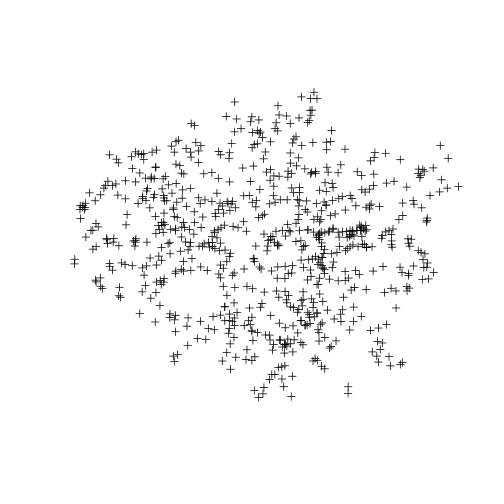
\includegraphics{figure/The_clipped_stations_dataset.png}
\caption{The clipped stations dataset}
\end{figure}

As the figure shows, only stations within the London boroughs are now
shown.

The \emph{third} way to achieve the same result uses the \texttt{rgeos}
package. This is more complex and not included in this tutorial
(interested readers can see a vignette of this, to accompany the
tutorial on
\href{http://rpubs.com/RobinLovelace/11796}{RPubs.com/Robinlovelace}).
The next section demonstrates spatial aggregation, a more advanced
version of spatial subsetting.

\subsection{Spatial aggregation}

As with R's very terse code for spatial subsetting, the base function
\texttt{aggregate} (which provides summaries of variables based on some
grouping variable) also behaves differently when the inputs are spatial
objects.

\begin{Shaded}
\begin{Highlighting}[]
\NormalTok{stations.c <- }\KeywordTok{aggregate}\NormalTok{(stations, lnd, length)}
\NormalTok{stations.c@data[, }\DecValTok{1}\NormalTok{]}
\end{Highlighting}
\end{Shaded}
\begin{verbatim}
##  [1] 48 22 43 18 12 13 25 24 12 46 18 20 28 32 38 19 30 25 31  7 10 38 12
## [24] 16 28 17 16 28  4  6 14 26  5
\end{verbatim}
The above code performs a number of steps in just one line:

\begin{itemize}
\item
  \texttt{aggregate} identifies which \texttt{lnd} polygon (borough)
  each \texttt{station} is located in and groups them accordingly
\item
  it counts the number of stations in each borough
\item
  a new spatial object is created and assigned the name
  \texttt{stations.c}, the count of stations
\end{itemize}
As shown below, the spatial implementation of \texttt{aggregate} can
provide summary statistics of variables. In this case we take the
variable \texttt{NUMBER} and find its mean value for the stations in
each ward.

\begin{Shaded}
\begin{Highlighting}[]
\NormalTok{stations.m <- }\KeywordTok{aggregate}\NormalTok{(stations[}\KeywordTok{c}\NormalTok{(}\StringTok{"NUMBER"}\NormalTok{)], }\DataTypeTok{by =} \NormalTok{lnd, }\DataTypeTok{FUN =} \NormalTok{mean)}
\end{Highlighting}
\end{Shaded}
For an optional advanced task, let us analyse and plot the result.

\begin{Shaded}
\begin{Highlighting}[]
\NormalTok{q <- }\KeywordTok{cut}\NormalTok{(stations.m$NUMBER, }\DataTypeTok{breaks =} \KeywordTok{c}\NormalTok{(}\KeywordTok{quantile}\NormalTok{(stations.m$NUMBER)), }\DataTypeTok{include.lowest =} \NormalTok{T)}
\KeywordTok{summary}\NormalTok{(q)}
\end{Highlighting}
\end{Shaded}
\begin{verbatim}
## [1.82e+04,1.94e+04] (1.94e+04,1.99e+04] (1.99e+04,2.05e+04] 
##                   9                   8                   8 
##  (2.05e+04,2.1e+04] 
##                   8
\end{verbatim}
\begin{Shaded}
\begin{Highlighting}[]
\NormalTok{clr <- }\KeywordTok{as.character}\NormalTok{(}\KeywordTok{factor}\NormalTok{(q, }\DataTypeTok{labels =} \KeywordTok{paste0}\NormalTok{(}\StringTok{"grey"}\NormalTok{, }\KeywordTok{seq}\NormalTok{(}\DecValTok{20}\NormalTok{, }\DecValTok{80}\NormalTok{, }\DecValTok{20}\NormalTok{))))}
\KeywordTok{plot}\NormalTok{(stations.m, }\DataTypeTok{col =} \NormalTok{clr)}
\KeywordTok{legend}\NormalTok{(}\DataTypeTok{legend =} \KeywordTok{paste0}\NormalTok{(}\StringTok{"q"}\NormalTok{, }\DecValTok{1}\NormalTok{:}\DecValTok{4}\NormalTok{), }\DataTypeTok{fill =} \KeywordTok{paste0}\NormalTok{(}\StringTok{"grey"}\NormalTok{, }\KeywordTok{seq}\NormalTok{(}\DecValTok{20}\NormalTok{, }\DecValTok{80}\NormalTok{, }\DecValTok{20}\NormalTok{)), }\StringTok{"topright"}\NormalTok{)}
\end{Highlighting}
\end{Shaded}
\begin{figure}[htbp]
\centering
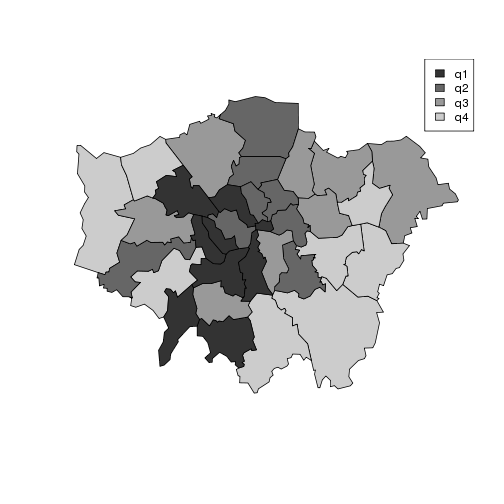
\includegraphics{figure/Choropleth_map_of_mean_values_of_stations_in_each_borough.png}
\caption{Choropleth map of mean values of stations in each
borough}
\end{figure}

\begin{Shaded}
\begin{Highlighting}[]
\NormalTok{areas <- }\KeywordTok{sapply}\NormalTok{(stations.m@polygons, function(x) x@area)}
\end{Highlighting}
\end{Shaded}
This results in a simple choropleth map and a new vector containing the
area of each borough. As an additional step, try comparing the mean area
of each borough with the mean value of stations within it:
\texttt{plot(stations.m\$NUMBER, areas)}.

\subsection{Optional advanced task: aggregation with gIntersects}

As with clipping, we can also do spatial aggregation with the rgeos
package. In some ways, this method makes explicit the steps taken in
\texttt{aggregate} `under the hood'. The code is quite involved and
intimidating, so feel free to skip this stage. Working through and
thinking about it this alternative method may, however, yield dividends
if you intend to perform more sophisticated spatial analysis in R.

\begin{Shaded}
\begin{Highlighting}[]
\KeywordTok{library}\NormalTok{(rgeos)}
\end{Highlighting}
\end{Shaded}
\begin{verbatim}
## rgeos version: 0.2-19, (SVN revision 394)
##  GEOS runtime version: 3.3.8-CAPI-1.7.8 
##  Polygon checking: TRUE
\end{verbatim}
\begin{Shaded}
\begin{Highlighting}[]
\NormalTok{int <- }\KeywordTok{gIntersects}\NormalTok{(stations, lnd, }\DataTypeTok{byid =} \OtherTok{TRUE}\NormalTok{)  }\CommentTok{# re-run the intersection query }
\KeywordTok{head}\NormalTok{(}\KeywordTok{apply}\NormalTok{(int, }\DataTypeTok{MARGIN =} \DecValTok{2}\NormalTok{, }\DataTypeTok{FUN =} \NormalTok{which))}
\NormalTok{b.indexes <- }\KeywordTok{which}\NormalTok{(int, }\DataTypeTok{arr.ind =} \OtherTok{TRUE}\NormalTok{)}
\KeywordTok{summary}\NormalTok{(b.indexes)}
\NormalTok{b.names <- lnd$name[b.indexes[, }\DecValTok{1}\NormalTok{]]}
\NormalTok{b.count <- }\KeywordTok{aggregate}\NormalTok{(b.indexes ~ b.names, }\DataTypeTok{FUN =} \NormalTok{length)}
\KeywordTok{head}\NormalTok{(b.count)}
\end{Highlighting}
\end{Shaded}
The above code first extracts the index of the row (borough) for which
the corresponding column is true and then converts this into names. The
final object created, \texttt{b.count} contains the number of station
points in each zone. According to this, Barking and Dagenham should
contain 12 station points. It is important to check the output makes
sense at every stage with R, so let's check to see this is indeed the
case with a quick plot:

\begin{Shaded}
\begin{Highlighting}[]
\KeywordTok{plot}\NormalTok{(lnd[}\KeywordTok{which}\NormalTok{(}\KeywordTok{grepl}\NormalTok{(}\StringTok{"Barking"}\NormalTok{, lnd$name)), ])}
\KeywordTok{points}\NormalTok{(stations)}
\end{Highlighting}
\end{Shaded}
\begin{figure}[htbp]
\centering
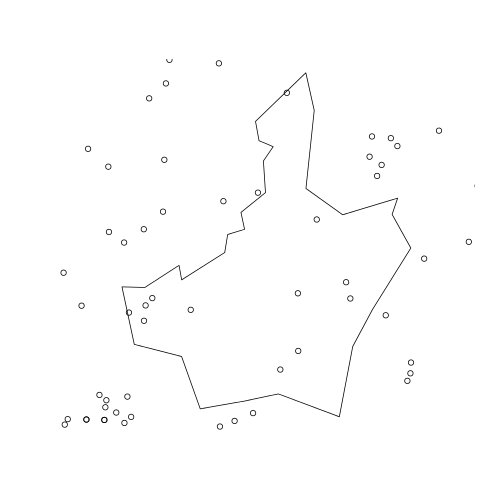
\includegraphics{figure/Train/tube_stations_in_Barking_and_Dagenham.png}
\caption{Train/tube stations in Barking and Dagenham}
\end{figure}

Now the fun part: count the points in the polygon and report back how
many there are!

We have now seen how to load, join and clip data. The second half of
this tutorial is concerned with \emph{visualisation} of the results. For
this, we will use ggplot2 and begin by looking at how it handles
non-spatial data.

\section{ggplot2}

This next section introduces a slightly different method of creating
plots in R using the \href{http://ggplot2.org/}{ggplot2 package}. The
package is an implementation of the Grammar of Graphics (Wilkinson 2005)
- a general scheme for data visualisation that breaks up graphs into
semantic components such as scales and layers. ggplot2 can serve as a
replacement for the base graphics in R (the functions you have been
plotting with today) and contains a number of default options that match
good visualisation practice.

The maps we produce will not be that meaningful - the focus here is on
sound visualisation with R and not sound analysis (obviously the value
of the former diminished in the absence of the latter!) Whilst the
instructions are step by step you are encouraged to deviate from them
(trying different colours for example) to get a better understanding of
what we are doing.

\texttt{ggplot2} is one of the best documented packages in R. The full
documentation for it can be found online and it is recommended you test
out the examples on your own machines and play with them:
http://docs.ggplot2.org/current/ .

Good examples of graphs can also be found on the website
\href{http://www.cookbook-r.com/Graphs/}{cookbook-r.com}.

Load the package:

\begin{Shaded}
\begin{Highlighting}[]
\KeywordTok{library}\NormalTok{(ggplot2)}
\end{Highlighting}
\end{Shaded}
It is worth noting that the basic \texttt{plot()} function requires no
data preparation but additional effort in colour selection/adding the
map key etc. \texttt{qplot()} and \texttt{ggplot()} (from the ggplot2
package) require some additional steps to format the spatial data but
select colours and add keys etc. automatically. More on this later.

As a first attempt with ggplot2 we can create a scatter plot with the
attribute data in the `sport' object created above. Type:

\begin{Shaded}
\begin{Highlighting}[]
\NormalTok{p <- }\KeywordTok{ggplot}\NormalTok{(sport@data, }\KeywordTok{aes}\NormalTok{(Partic_Per, Pop_2001))}
\end{Highlighting}
\end{Shaded}
What you have just done is set up a ggplot object where you say where
you want the input data to come from. \texttt{sport@data} is actually a
data frame contained within the wider spatial object \texttt{sport} (the
\texttt{@} enables you to access the attribute table of the sport
shapefile). The characters inside the \texttt{aes} argument refer to the
parts of that data frame you wish to use (the variables
\texttt{Partic\_Per} and \texttt{Pop\_2001}). This has to happen within
the brackets of \texttt{aes()}, which means, roughly speaking
`aesthetics that vary'.

If you just type p and hit enter you get the error
\texttt{No layers in plot}. This is because you have not told ggplot
what you want to do with the data. We do this by adding so-called
``geoms'', in this case \texttt{geom\_point()}.

\begin{Shaded}
\begin{Highlighting}[]
\NormalTok{p + }\KeywordTok{geom_point}\NormalTok{()}
\end{Highlighting}
\end{Shaded}
\begin{figure}[htbp]
\centering
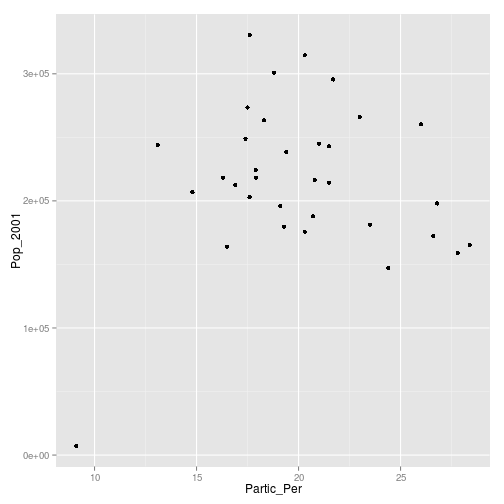
\includegraphics{figure/A_simple_ggplot.png}
\caption{A simple ggplot}
\end{figure}

Within the brackets you can alter the nature of the points. Try
something like \texttt{p + geom\_point(colour = "red", size=2)} and
experiment.

If you want to scale the points by borough population and colour them by
sports participation this is also fairly easy by adding another
\texttt{aes()} argument.

\begin{Shaded}
\begin{Highlighting}[]
\NormalTok{p + }\KeywordTok{geom_point}\NormalTok{(}\KeywordTok{aes}\NormalTok{(}\DataTypeTok{colour =} \NormalTok{Partic_Per, }\DataTypeTok{size =} \NormalTok{Pop_2001))}
\end{Highlighting}
\end{Shaded}
The real power of ggplot2 lies in its ability to add layers to a plot.
In this case we can add text to the plot.

\begin{Shaded}
\begin{Highlighting}[]
\NormalTok{p + }\KeywordTok{geom_point}\NormalTok{(}\KeywordTok{aes}\NormalTok{(}\DataTypeTok{colour =} \NormalTok{Partic_Per, }\DataTypeTok{size =} \NormalTok{Pop_2001)) + }\KeywordTok{geom_text}\NormalTok{(}\DataTypeTok{size =} \DecValTok{2}\NormalTok{, }
    \KeywordTok{aes}\NormalTok{(}\DataTypeTok{label =} \NormalTok{name))}
\end{Highlighting}
\end{Shaded}
\begin{figure}[htbp]
\centering
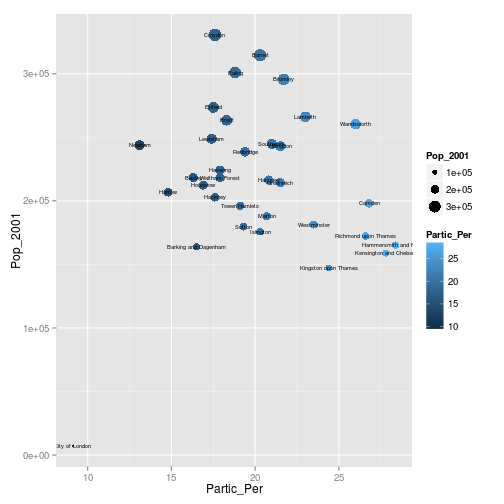
\includegraphics{figure/ggplot_for_text.png}
\caption{ggplot for text}
\end{figure}

This idea of layers (or geoms) is quite different from the standard plot
functions in R, but you will find that each of the functions does a lot
of clever stuff to make plotting much easier (see the documentation for
a full list).

The following steps will create a map to show the percentage of the
population in each London Borough who regularly participate in sports
activities.

\subsection{``Fortifying'' spatial objects for ggplot}

To get the shapefiles into a format that can be plotted we have to use
the \texttt{fortify()} function. Spatial objects in R have a number of
slots containing the various items of data (polygon geometry,
projection, attribute information) associated with a shapefile. Slots
can be thought of as shelves within the data object that contain the
different attributes. The ``polygons'' slot contains the geometry of the
polygons in the form of the XY coordinates used to draw the polygon
outline. The generic plot function can work out what to do with these,
ggplot2 cannot. We therefore need to extract them as a data frame. The
fortify function was written specifically for this purpose. For this to
work, either \texttt{gpclib} or \texttt{rgeos} packages must be
installed.

\begin{Shaded}
\begin{Highlighting}[]
\CommentTok{# library(gpclib); gpclibPermit() # uncomment if rgeos not installed}
\NormalTok{sport.f <- }\KeywordTok{fortify}\NormalTok{(sport, }\DataTypeTok{region =} \StringTok{"ons_label"}\NormalTok{)}
\end{Highlighting}
\end{Shaded}
This step has lost the attribute information associated with the sport
object. We can add it back using the merge function (this performs a
data join). To find out how this function works look at the output of
typing \texttt{?merge}.

\begin{Shaded}
\begin{Highlighting}[]
\NormalTok{sport.f <- }\KeywordTok{merge}\NormalTok{(sport.f, sport@data, }\DataTypeTok{by.x =} \StringTok{"id"}\NormalTok{, }\DataTypeTok{by.y =} \StringTok{"ons_label"}\NormalTok{)}
\end{Highlighting}
\end{Shaded}
Take a look at the \texttt{sport.f} object to see its contents. You
should see a large data frame containing the latitude and longitude
(they are actually Easting and Northing as the data are in British
National Grid format) coordinates alongside the attribute information
associated with each London Borough. If you type \texttt{print(sport.f)}
you will see just how many coordinate pairs are required! To keep the
output to a minimum, take a peek at the object using just the
\texttt{head} command:

\begin{Shaded}
\begin{Highlighting}[]
\KeywordTok{head}\NormalTok{(sport.f[, }\DecValTok{1}\NormalTok{:}\DecValTok{8}\NormalTok{])}
\end{Highlighting}
\end{Shaded}
\begin{verbatim}
##     id   long    lat order  hole piece  group           name
## 1 00AA 531027 181611     1 FALSE     1 00AA.1 City of London
## 2 00AA 531555 181659     2 FALSE     1 00AA.1 City of London
## 3 00AA 532136 182198     3 FALSE     1 00AA.1 City of London
## 4 00AA 532946 181895     4 FALSE     1 00AA.1 City of London
## 5 00AA 533411 182038     5 FALSE     1 00AA.1 City of London
## 6 00AA 533843 180794     6 FALSE     1 00AA.1 City of London
\end{verbatim}
\subsection{Maps in ggplot2}

It is now straightforward to produce a map using all the built in tools
(such as setting the breaks in the data) that ggplot2 has to offer.
\texttt{coord\_equal()} is the equivalent of asp=T in regular plots with
R:

\begin{Shaded}
\begin{Highlighting}[]
\NormalTok{Map <- }\KeywordTok{ggplot}\NormalTok{(sport.f, }\KeywordTok{aes}\NormalTok{(long, lat, }\DataTypeTok{group =} \NormalTok{group, }\DataTypeTok{fill =} \NormalTok{Partic_Per)) + }\KeywordTok{geom_polygon}\NormalTok{() + }
    \KeywordTok{coord_equal}\NormalTok{() + }\KeywordTok{labs}\NormalTok{(}\DataTypeTok{x =} \StringTok{"Easting (m)"}\NormalTok{, }\DataTypeTok{y =} \StringTok{"Northing (m)"}\NormalTok{, }\DataTypeTok{fill =} \StringTok{"% Sport Partic."}\NormalTok{) + }
    \KeywordTok{ggtitle}\NormalTok{(}\StringTok{"London Sports Participation"}\NormalTok{)}
\end{Highlighting}
\end{Shaded}
Now, just typing \texttt{Map} should result in your first ggplot-made
map of London! There is a lot going on in the code above, so think about
it line by line: what have each of the elements of code above been
designed to do? Also note how the \texttt{aes()} components can be
combined into one set of brackets after \texttt{ggplot}, that has
relevance for all layers, rather than being broken into separate parts
as we did above. The different plot functions still know what to do with
these. The \texttt{group=group} points ggplot to the group column added
by \texttt{fortify()} and it identifies the groups of coordinates that
pertain to individual polygons (in this case London Boroughs).

The default colours are really nice but we may wish to produce the map
in black and white, which should produce a map like that shown below
(and try changing the colors):

\begin{Shaded}
\begin{Highlighting}[]
\NormalTok{Map + }\KeywordTok{scale_fill_gradient}\NormalTok{(}\DataTypeTok{low =} \StringTok{"white"}\NormalTok{, }\DataTypeTok{high =} \StringTok{"black"}\NormalTok{)}
\end{Highlighting}
\end{Shaded}
\begin{figure}[htbp]
\centering
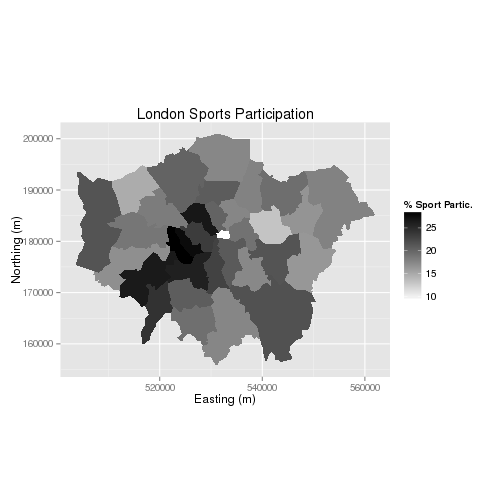
\includegraphics{figure/Greyscale_map.png}
\caption{Greyscale map}
\end{figure}

Saving plot images is also easy. You just need to use \texttt{ggsave}
after each plot, e.g. \texttt{ggsave("my\_map.pdf")} will save the map
as a pdf, with default settings. For a larger map, you could try the
following:

\begin{Shaded}
\begin{Highlighting}[]
\KeywordTok{ggsave}\NormalTok{(}\StringTok{"my_large_plot.png"}\NormalTok{, }\DataTypeTok{scale =} \DecValTok{3}\NormalTok{, }\DataTypeTok{dpi =} \DecValTok{400}\NormalTok{)}
\end{Highlighting}
\end{Shaded}
\section{Adding base maps to ggplot2 with ggmap}

\href{http://journal.r-project.org/archive/2013-1/kahle-wickham.pdf}{ggmap}
is a package that uses the ggplot2 syntax as a template to create maps
with image tiles taken from map servers such as Google and
\href{http://www.openstreetmap.org/}{OpenStreetMap}:

\begin{Shaded}
\begin{Highlighting}[]
\KeywordTok{library}\NormalTok{(ggmap)  }\CommentTok{# you may have to use install.packages to install it first}
\end{Highlighting}
\end{Shaded}
The \texttt{sport} object loaded previously is in British National Grid
but the ggmap image tiles are in WGS84. We therefore need to use the
sport.wgs84 object created in the reprojection operation earlier.

The first job is to calculate the bounding box (bb for short) of the
sport.wgs84 object to identify the geographic extent of the image tiles
that we need.

\begin{Shaded}
\begin{Highlighting}[]
\NormalTok{b <- }\KeywordTok{bbox}\NormalTok{(sport.wgs84)}
\NormalTok{b[}\DecValTok{1}\NormalTok{, ] <- (b[}\DecValTok{1}\NormalTok{, ] - }\KeywordTok{mean}\NormalTok{(b[}\DecValTok{1}\NormalTok{, ])) * }\FloatTok{1.05} \NormalTok{+ }\KeywordTok{mean}\NormalTok{(b[}\DecValTok{1}\NormalTok{, ])}
\NormalTok{b[}\DecValTok{2}\NormalTok{, ] <- (b[}\DecValTok{2}\NormalTok{, ] - }\KeywordTok{mean}\NormalTok{(b[}\DecValTok{2}\NormalTok{, ])) * }\FloatTok{1.05} \NormalTok{+ }\KeywordTok{mean}\NormalTok{(b[}\DecValTok{2}\NormalTok{, ])}
\CommentTok{# scale longitude and latitude (increase bb by 5% for plot) replace 1.05}
\CommentTok{# with 1.xx for an xx% increase in the plot size}
\end{Highlighting}
\end{Shaded}
This is then fed into the \texttt{get\_map} function as the location
parameter. The syntax below contains 2 functions. \texttt{ggmap} is
required to produce the plot and provides the base map data.

\begin{Shaded}
\begin{Highlighting}[]
\NormalTok{lnd.b1 <- }\KeywordTok{ggmap}\NormalTok{(}\KeywordTok{get_map}\NormalTok{(}\DataTypeTok{location =} \NormalTok{b))}
\end{Highlighting}
\end{Shaded}
\begin{verbatim}
## Warning: bounding box given to google - spatial extent only approximate.
\end{verbatim}
In much the same way as we did above we can then layer the plot with
different geoms.

First fortify the sport.wgs84 object and then merge with the required
attribute data (we already did this step to create the sport.f object).

\begin{Shaded}
\begin{Highlighting}[]
\NormalTok{sport.wgs84.f <- }\KeywordTok{fortify}\NormalTok{(sport.wgs84, }\DataTypeTok{region =} \StringTok{"ons_label"}\NormalTok{)}
\NormalTok{sport.wgs84.f <- }\KeywordTok{merge}\NormalTok{(sport.wgs84.f, sport.wgs84@data, }\DataTypeTok{by.x =} \StringTok{"id"}\NormalTok{, }\DataTypeTok{by.y =} \StringTok{"ons_label"}\NormalTok{)}
\end{Highlighting}
\end{Shaded}
We can now overlay this on our base map.

\begin{Shaded}
\begin{Highlighting}[]
\NormalTok{lnd.b1 + }\KeywordTok{geom_polygon}\NormalTok{(}\DataTypeTok{data =} \NormalTok{sport.wgs84.f, }\KeywordTok{aes}\NormalTok{(}\DataTypeTok{x =} \NormalTok{long, }\DataTypeTok{y =} \NormalTok{lat, }\DataTypeTok{group =} \NormalTok{group, }
    \DataTypeTok{fill =} \NormalTok{Partic_Per), }\DataTypeTok{alpha =} \FloatTok{0.5}\NormalTok{)}
\end{Highlighting}
\end{Shaded}
The code above contains a lot of parameters. Use the ggplot2 help pages
to find out what they are. The resulting map looks okay, but it would be
improved with a simpler base map in black and white. A design firm
called stamen provide the tiles we need and they can be brought into the
plot with the \texttt{get\_map} function:

\begin{Shaded}
\begin{Highlighting}[]
\NormalTok{lnd.b2 <- }\KeywordTok{ggmap}\NormalTok{(}\KeywordTok{get_map}\NormalTok{(}\DataTypeTok{location =} \NormalTok{b, }\DataTypeTok{source =} \StringTok{"stamen"}\NormalTok{, }\DataTypeTok{maptype =} \StringTok{"toner"}\NormalTok{, }
    \DataTypeTok{crop =} \OtherTok{TRUE}\NormalTok{))}
\end{Highlighting}
\end{Shaded}
We can then produce the plot as before.

\begin{Shaded}
\begin{Highlighting}[]
\NormalTok{lnd.b2 + }\KeywordTok{geom_polygon}\NormalTok{(}\DataTypeTok{data =} \NormalTok{sport.wgs84.f, }\KeywordTok{aes}\NormalTok{(}\DataTypeTok{x =} \NormalTok{long, }\DataTypeTok{y =} \NormalTok{lat, }\DataTypeTok{group =} \NormalTok{group, }
    \DataTypeTok{fill =} \NormalTok{Partic_Per), }\DataTypeTok{alpha =} \FloatTok{0.5}\NormalTok{)}
\end{Highlighting}
\end{Shaded}
Finally, if we want to increase the detail of the base map, get\_map has
a zoom parameter.

\begin{Shaded}
\begin{Highlighting}[]
\NormalTok{lnd.b3 <- }\KeywordTok{ggmap}\NormalTok{(}\KeywordTok{get_map}\NormalTok{(}\DataTypeTok{location =} \NormalTok{b, }\DataTypeTok{source =} \StringTok{"stamen"}\NormalTok{, }\DataTypeTok{maptype =} \StringTok{"toner"}\NormalTok{, }
    \DataTypeTok{crop =} \OtherTok{TRUE}\NormalTok{, }\DataTypeTok{zoom =} \DecValTok{11}\NormalTok{))}

\NormalTok{lnd.b3 + }\KeywordTok{geom_polygon}\NormalTok{(}\DataTypeTok{data =} \NormalTok{sport.wgs84.f, }\KeywordTok{aes}\NormalTok{(}\DataTypeTok{x =} \NormalTok{long, }\DataTypeTok{y =} \NormalTok{lat, }\DataTypeTok{group =} \NormalTok{group, }
    \DataTypeTok{fill =} \NormalTok{Partic_Per), }\DataTypeTok{alpha =} \FloatTok{0.5}\NormalTok{)}
\end{Highlighting}
\end{Shaded}
\begin{figure}[htbp]
\centering
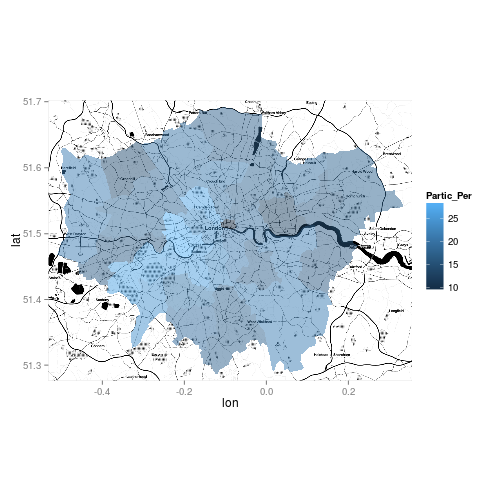
\includegraphics{figure/Basemap_3.png}
\caption{Basemap 3}
\end{figure}

\section{Advanced Task: Faceting for Maps}

\begin{Shaded}
\begin{Highlighting}[]
\KeywordTok{library}\NormalTok{(reshape2)  }\CommentTok{# this may not be installed. }
\CommentTok{# If not install it, or skip the next two steps…}
\end{Highlighting}
\end{Shaded}
Load the data - this shows historic population values between 1801 and
2001 for London, again from the London data store.

\begin{Shaded}
\begin{Highlighting}[]
\NormalTok{london.data <- }\KeywordTok{read.csv}\NormalTok{(}\StringTok{"data/census-historic-population-borough.csv"}\NormalTok{)}
\end{Highlighting}
\end{Shaded}
``Melt'' the data so that the columns become rows.

\begin{Shaded}
\begin{Highlighting}[]
\NormalTok{london.data.melt <- }\KeywordTok{melt}\NormalTok{(london.data, }\DataTypeTok{id =} \KeywordTok{c}\NormalTok{(}\StringTok{"Area.Code"}\NormalTok{, }\StringTok{"Area.Name"}\NormalTok{))}
\end{Highlighting}
\end{Shaded}
Only do this step if reshape and melt failed

\begin{Shaded}
\begin{Highlighting}[]
\NormalTok{london.data.melt <- }\KeywordTok{read.csv}\NormalTok{(}\StringTok{"london_data_melt.csv"}\NormalTok{)}
\end{Highlighting}
\end{Shaded}
Merge the population data with the London borough geometry contained
within our sport.f object.

\begin{Shaded}
\begin{Highlighting}[]
\NormalTok{plot.data <- }\KeywordTok{merge}\NormalTok{(sport.f, london.data.melt, }\DataTypeTok{by.x =} \StringTok{"id"}\NormalTok{, }\DataTypeTok{by.y =} \StringTok{"Area.Code"}\NormalTok{)}
\end{Highlighting}
\end{Shaded}
Reorder this data (ordering is important for plots).

\begin{Shaded}
\begin{Highlighting}[]
\NormalTok{plot.data <- plot.data[}\KeywordTok{order}\NormalTok{(plot.data$order), ]}
\end{Highlighting}
\end{Shaded}
We can now use faceting to produce one map per year (this may take a
little while to appear).

\begin{Shaded}
\begin{Highlighting}[]
\KeywordTok{ggplot}\NormalTok{(}\DataTypeTok{data =} \NormalTok{plot.data, }\KeywordTok{aes}\NormalTok{(}\DataTypeTok{x =} \NormalTok{long, }\DataTypeTok{y =} \NormalTok{lat, }\DataTypeTok{fill =} \NormalTok{value, }\DataTypeTok{group =} \NormalTok{group)) + }
    \KeywordTok{geom_polygon}\NormalTok{() + }\KeywordTok{geom_path}\NormalTok{(}\DataTypeTok{colour =} \StringTok{"grey"}\NormalTok{, }\DataTypeTok{lwd =} \FloatTok{0.1}\NormalTok{) + }\KeywordTok{coord_equal}\NormalTok{() + }
    \KeywordTok{facet_wrap}\NormalTok{(~variable)}
\end{Highlighting}
\end{Shaded}
\begin{figure}[htbp]
\centering
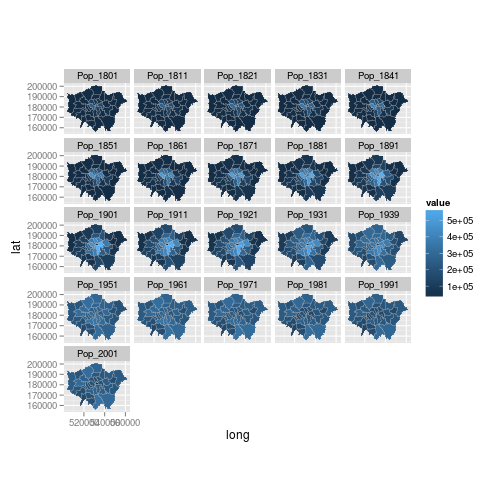
\includegraphics{figure/Faceted_map.png}
\caption{Faceted map}
\end{figure}

Again there is a lot going on here so explore the documentation to make
sure you understand it. Try out different colour values as well.

Add a title and replace the axes names with ``easting'' and ``northing''
and save your map as a pdf.

\section{Taking spatial data analysis in R further}

The skills you have learned in this tutorial are applicable to a very
wide range of datasets, spatial or not. Often experimentation is the
most rewarding learning method, rather than just searching for the
`best' way of doing something (Kabakoff, 2011). We recommend you play
around with your own data.

If you would like to learn more about R's spatial functionalities,
including more exercises on loading, saving and manipulating data, we
recommend a slightly longer and more advanced tutorial (Cheshire and
Lovelace, 2014). An up-to-date repository of this project, including
example dataset and all the code used to compile the tutorial, can be
found on its GitHub page:
\href{https://github.com/geocomPP/sdvwR}{github.com/geocomPP/sdvwR} .
Such lengthy tutorials are worth doing to think about spatial data in R
systematically, rather than seeing R as a discrete collection of
functions. In R the whole is greater than the sum of its parts.

The supportive online communities surrounding large open source programs
such as R are one of their greatest assets, so we recommend you become
an active
``\href{http://blog.cleverelephant.ca/2013/10/being-open-source-citizen.html}{open
source citizen}'' rather than a passive consumer (Ramsey \& Dubovsky,
2013).

This does not necessarily mean writing R source code - it can simply
mean helping others use R. We therefore conclude the tutorial with a
list of resources that will help you further sharpen you R skills, find
help and contribute to the growing online R community:

\begin{itemize}
\item
  R's homepage hosts a wealth of
  \href{http://cran.r-project.org/manuals.html}{official} and
  \href{http://cran.r-project.org/other-docs.html}{contributed} guides.
\item
  Stack Exchange and GIS Stack Exchange groups - try searching for
  ``{[}R{]}''. If your issue has not been not been addressed yet, you
  could post a polite question.
\item
  R's \href{http://www.r-project.org/mail.html}{mailing lists} - the
  R-sig-geo list may be of particular interest here.
\end{itemize}
Books: despite the strength of R's online community, nothing beats a
physical book for concentrated learning. We would particularly recommend
the following:

\begin{itemize}
\item
  ggplot2: elegant graphics for data analysis (Wickham 2009)
\item
  Bivand et al. (2013) Provide a dense and detailed overview of spatial
  data analysis in an updated version of the book by the developers of
  many of R's spatial functions.
\item
  Kabacoff (2011) is a more general R book; it has many fun worked
  examples.
\end{itemize}
\newpage \section{References}

Bivand, R. S., Pebesma, E. J., \& Rubio, V. G. (2008). Applied spatial
data: analysis with R. Springer.

Cheshire, J. \& Lovelace, R. (2014). Manipulating and visualizing
spatial data with R. Book chapter in Press.

Harris, R. (2012). A Short Introduction to R.
\href{http://www.social-statistics.org/}{social-statistics.org}.

Johnson, P. E. (2013). R Style. An Rchaeological Commentary. The
Comprehensive R Archive Network.

Kabacoff, R. (2011). R in Action. Manning Publications Co.

Ramsey, P., \& Dubovsky, D. (2013). Geospatial Software's Open Future.
GeoInformatics, 16(4).

Torfs and Brauer (2012). A (very) short Introduction to R. The
Comprehensive R Archive Network.

Wickham, H. (2009). ggplot2: elegant graphics for data analysis.
Springer.

Wilkinson, L. (2005). The grammar of graphics. Springer.

\begin{Shaded}
\begin{Highlighting}[]
\KeywordTok{source}\NormalTok{(}\StringTok{"latex/rmd2pdf.R"}\NormalTok{)  }\CommentTok{# convert .Rmd to .tex file}
\end{Highlighting}
\end{Shaded}

\end{document}
